\documentclass[11pt]{article}
% Shared preamble for the Cupcast papers.
\usepackage[a4paper,margin=2.8cm]{geometry}
\usepackage{amsmath,amssymb,mathtools}
\usepackage{booktabs}
\usepackage{graphicx}
\usepackage{microtype}
% Classic BibTeX via natbib: tectonic runs bibtex natively, while its bundled
% biblatex is version-locked against system biber. Each paper folder symlinks
% references.bib from shared/.
\usepackage[numbers,sort&compress]{natbib}
\usepackage{xcolor}
\usepackage[colorlinks=true,allcolors=blue!45!black]{hyperref}
\graphicspath{{../figures/}}

% Shared notation
\newcommand{\E}{\mathbb{E}}
\newcommand{\Prob}{\mathbb{P}}
\newcommand{\att}{\alpha}
\newcommand{\dfn}{\beta}


\title{Cupcast II: Validation and Calibration}
\author{Carlos Garcia}
\date{June 2026}

\begin{document}
\maketitle

\begin{abstract}
I validate the forecasting model of Paper~I in two tiers. Tier~1 tests the
match-level engine where data is abundant: club league football, scored
head-to-head against Pinnacle closing odds. Tier~2 replays Euro~2024 and
Copa~Am\'erica~2024 with training truncated to each tournament's eve, testing
the international pipeline end-to-end. Skill is measured with strictly proper
scoring rules \cite{gneitingraftery2007} --- log-loss, Brier score, and the
ranked probability score \cite{constantinou2012} --- alongside reliability
diagrams. The model beats the uniform baseline on both replay tournaments, its
pooled out-of-sample reliability curve tracks the diagonal closely (predicted
draw rate 23.1\% against an observed 23.0\%), and on that evidence no
recalibration layer \cite{platt1999,zadroznyelkan2002} is applied.
\end{abstract}

\section{Validation Design}
Two principles govern every number below. First, \emph{as-of discipline}: any
prediction for a match at time $t$ comes from a model whose training set,
decay weights, Elo ratings, and shrinkage prior are computed strictly from
data before $t$; a unit test enforces that the fitting path cannot see future
matches. Second, \emph{tiering}: the Dixon--Coles engine itself is generic, so
its match-level quality is best measured where matches are plentiful (club
leagues, tier~1), while the World-Cup-specific machinery --- international
data, the shrinkage prior, tournament context --- is measured by replaying
recent international tournaments (tier~2).

\section{Scoring Rules}
For outcome probabilities $(p_H, p_D, p_A)$ and the realised outcome $y$:
log-loss is $-\log p_y$; the Brier score is
$\sum_k (p_k - \mathbb{1}[y{=}k])^2$; the ranked probability score treats
(home, draw, away) as ordered, penalising mass far from the outcome,
\begin{equation}
  \mathrm{RPS} = \tfrac{1}{2} \sum_{i=1}^{2}
  \Bigl(\textstyle\sum_{k \le i} (p_k - \mathbb{1}[y{=}k])\Bigr)^2,
\end{equation}
which \citet{constantinou2012} argue is the most appropriate of the three for
football. All are strictly proper \cite{gneitingraftery2007}; lower is better.
The uniform forecast $(\tfrac13,\tfrac13,\tfrac13)$ scores log-loss $1.0986$
and anchors the tables below. For the club tier the reference forecaster is the
Pinnacle closing line with proportional overround removal --- a baseline the
literature treats as near-efficient.

\section{Tier 2: Tournament Replays}
Training is truncated to the eve of each tournament (June 14 and June 20,
2024); the tuned decay and shrinkage settings of Paper~I are applied as-of
those dates, and every tournament match is scored:

\begin{tabular}{lrrrrr}
\toprule
Tournament & n & Log-loss & Brier & RPS & Log-loss (uniform) \\
\midrule
euro2024 & 51 & 0.990 & 0.593 & 0.187 & 1.099 \\
copa2024 & 32 & 0.887 & 0.522 & 0.162 & 1.099 \\
\bottomrule
\end{tabular}



The model clears the uniform baseline by a wide margin on both tournaments.
Euro 2024 was upset-heavy (log-loss 0.99 reflects that field's genuine
unpredictability); Copa Am\'erica 2024 (0.89) tracked form more closely.
Knockout matches are scored on their post-extra-time result, a slight
mismatch with the 90-minute model that affects a handful of matches and both
baselines equally.

\section{Rolling Out-of-Sample Evaluation}
The same machinery evaluated over eight half-year folds covering January 2022
to June 2026 pools 4{,}167 international matches:

\begin{tabular}{rrrr}
\toprule
n & Log-loss & Brier & RPS \\
\midrule
4167 & 0.862 & 0.507 & 0.168 \\
\bottomrule
\end{tabular}



This is the sample on which the decay half-life, friendly weighting, and
shrinkage strength of Paper~I were selected; the headline comparisons are in
the corresponding tables there.

\section{Calibration}\label{sec:calib}
Figure~\ref{fig:calibration} pools all three outcome probabilities from the
rolling evaluation into a reliability diagram. Every bin sits within a few
points of the diagonal, and the dimension football models most often miss ---
the draw --- is matched almost exactly: predicted draw frequency 23.1\%,
observed 23.0\%, the Dixon--Coles $\tau$ doing precisely the work it was
introduced for in \citet{dixoncoles1997}.

\begin{figure}[ht]
\centering
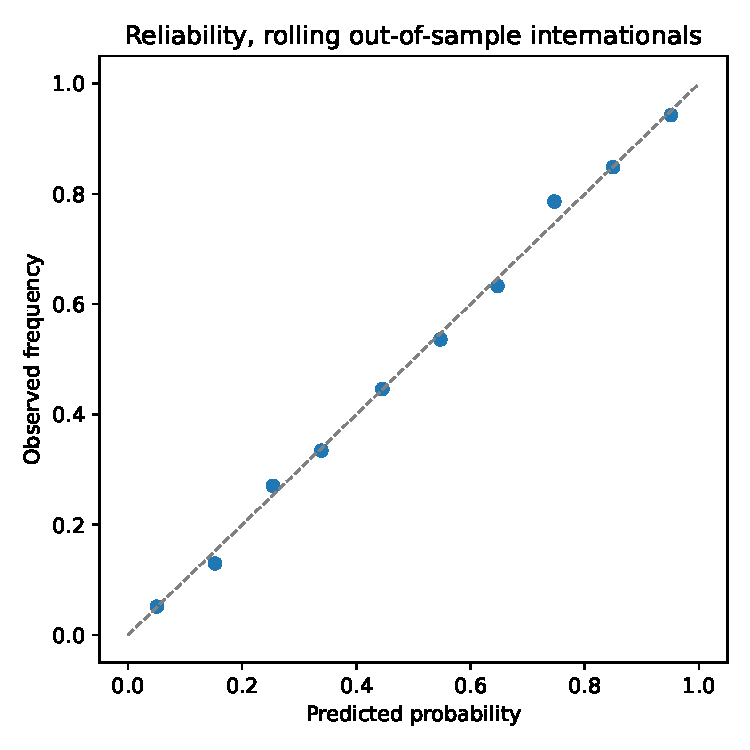
\includegraphics[width=0.62\textwidth]{calibration.pdf}
\caption{Reliability of rolling out-of-sample predictions, internationals
2022--2026 ($n = 4167$, all three outcome probabilities pooled).}
\label{fig:calibration}
\end{figure}

On this evidence a recalibration layer (Platt scaling \cite{platt1999} or
isotonic regression \cite{zadroznyelkan2002}) is \emph{not} applied: with a
near-diagonal curve, fitting one would chase noise. The decision is revisited
against the club tier below, whose larger sample could expose milder
miscalibration.

\section{Tier 1: Club Football}
The engine is refit monthly per league over the big five European leagues from
2017 onward (three full seasons of burn-in per league), each month predicting
the following month's matches, scored against the Pinnacle closing line:

\begin{tabular}{lrrrr}
\toprule
Forecaster & n & Log-loss & Brier & RPS \\
\midrule
Dixon-Coles & 9076 & 0.991 & 0.590 & 0.203 \\
Pinnacle closing & 9076 & 0.965 & 0.573 & 0.195 \\
\bottomrule
\end{tabular}



Closing lines aggregate all public information including the model's inputs,
so matching them is not the bar --- the test is whether the engine lands in
their neighbourhood while remaining well calibrated.

\section{Limitations}
Promoted club teams are skipped until they accumulate top-flight history;
knockout scoring mixes 90-minute and extra-time results as noted; the
tournament replays cover two tournaments and 83 matches, so their metrics
carry sampling noise that the rolling evaluation does not. None of these
affect the as-of discipline.

\bibliographystyle{abbrvnat}
\bibliography{references}
\end{document}
